% %%%%%%%%%%%%%%%%%%%%%%%%%%%%%%%%%%%%%%%%%%%%%%%%
% % Projeto de doutorado -- GAS UFSC -- Tex/LaTex 
% Autor: Eduardo Alberto Duarte Lacerda %
% Orientador: Roberto Cid Fernandes Jr.
% % 15/Feb/2015
% %%%%%%%%%%%%%%%%%%%%%%%%%%%%%%%%%%%%%%%%%%%%%%%%
\documentclass[a4paper,12pt]{article}

\usepackage[round,authoryear]{natbib}
\usepackage[utf8x]{inputenc} \usepackage[portuguese,brazilian]{babel}
\usepackage{aecompl}
\usepackage[table, usenames, dvipsnames]{xcolor}
\usepackage{color}
\usepackage{textcomp}
\usepackage{ctable}
\usepackage[T1]{fontenc}
\usepackage{mathrsfs}
% \PassOptionsToPackage{svgnames}{xcolor} \usepackage{listings} \usepackage{pdfpages}
\usepackage[colorlinks,linkcolor=black,bookmarks=true,citecolor=black]{hyperref}

% %% page geometry %%%
\usepackage{geometry}
\geometry{verbose,a4paper,tmargin=3cm,bmargin=2.5cm,
lmargin=2.5cm,rmargin=2cm,headsep=5mm,footskip=0cm}
% %%% page layout %%%%
\usepackage{fancyhdr}
\pagestyle{fancy}
\lhead{}\chead{}\rhead{}
\lfoot{}\cfoot{}\rfoot{}
\fancyhead{}
\rfoot{\thepage}

\newcommand{\mnras}{MNRAS}
\newcommand{\apj}{ApJ}
\newcommand{\pasp}{PASP}
\renewcommand{\it}{\textit}
\newcommand{\aj}{AJ}					%{The Astronomical Journal}
\newcommand{\apjs}{ApJS}

% \renewcommand{\footrulewidth}{.5pt}
\renewcommand{\headrulewidth}{0.0pt}
% \documentclass{nathesis}
\usepackage{xspace}
\usepackage{color}
\usepackage{float}

% ********************* Lacerda's Definitions ************************
\newcommand\pycasso{\textsc{p}y\textsc{casso}\xspace}
% \newcommand\pcalifa{\textsc{pca}lifa\xspace}
\newcommand\pcalifa{PCA\textsc{lifa}\xspace}
\newcommand{\meanL}[1]{\relax\ifmmode \langle #1 \rangle_L \else $\langle #1 \rangle_L$\xspace \fi}
\newcommand{\mean}[1]{\relax\ifmmode \langle #1 \rangle \else $\langle #1 \rangle$\xspace \fi}
\newcommand{\signature}[2][2.5in]{%
  \noindent%
  \begin{center}
  \begin{tabular}{@{}p{#1}@{}}
    \\ \hline \\ [-.75\normalbaselineskip]
    #2
  \end{tabular} 
  \end{center}
}
% *******************************************************************

% ********************* Andre's Definitions ************************
\def\starlight{\textsc{starlight}\xspace}      %smallcaps Starlight%
\def\starlightUV{\textsc{starlight+UV}\xspace} %smallcaps Starlight+UV%
\def\STARLIGHT{\textit{STARLIGHT}\xspace}                %Starlight%
\def\STARLIGHTUV{\textit{STARLIGHT+UV}\xspace}        %Starlight+UV%
% \def\SDSS{\textit{SDSS}\xspace}           %Sloan Digital Sky Survey%
\def\SDSS{SDSS\xspace}           %Sloan Digital Sky Survey% \def\galex{\textit{GALEX}\xspace}
\def\citneed{\textsuperscript{\bf \textcolor{red}{[citation needed]}}\xspace}
\def\fixme{\textsuperscript{\bf \textcolor{red}{[FIXME]}}\xspace} \def\Halpha{\ifmmode
\mathrm{H}\alpha \else H$\alpha$\xspace \fi} \def\WHa{\ifmmode W_{\mathrm{H}\alpha} \else
$W_{\mathrm{H}\alpha}$\xspace \fi} \def\Hbeta{\ifmmode \mathrm{H}\beta \else H$\beta$\xspace \fi}
\def\NII{[N\thinspace\textsc{ii}] $\lambda 6584$\xspace} \def\nII{\ifmmode [\mathrm{N\,\textsc{ii}}]
\else [N\thinspace\textsc{ii}]\xspace \fi} \def\WnII{W_{\mathrm{[N\,\textsc{ii}]}}}
\def\OIII{[O\thinspace\textsc{iii}] $\lambda 5007$\xspace} \def\oIII{\ifmmode
[\mathrm{O\,\textsc{iii}}] \else [O\thinspace{\sc iii}]\xspace \fi}
% ******************************************************************* I guess these are Cid's
% definitions. I have found them in Luis' masters thesis. Some of them are rather useful.
% ********************* CID'S DEFINITIONS **************************

\def\ojo{\fbox{\bf !$\odot$j$\odot$!}}      %Olho! Needs Correction%

% *******************************************************************

% Journals - from AASTex Natalia@UFSC - 16/Nov/2005
\def\aj{AJ}%
          % Astronomical Journal
\def\actaa{Acta Astron.}%
          % Acta Astronomica
\def\araa{ARA\&A}%
          % Annual Review of Astron and Astrophys
\def\apj{ApJ}%
          % Astrophysical Journal
\def\apjl{ApJ}%
          % Astrophysical Journal, Letters
\def\apjs{ApJS}%
          % Astrophysical Journal, Supplement
\def\ao{Appl.~Opt.}%
          % Applied Optics
\def\apss{Ap\&SS}%
          % Astrophysics and Space Science
\def\aap{A\&A}%
          % Astronomy and Astrophysics
\def\aapr{A\&A~Rev.}%
          % Astronomy and Astrophysics Reviews
\def\aaps{A\&AS}%
          % Astronomy and Astrophysics, Supplement
\def\azh{AZh}%
          % Astronomicheskii Zhurnal
\def\baas{BAAS}%
          % Bulletin of the AAS
\def\caa{Chinese Astron. Astrophys.}%
          % Chinese Astronomy and Astrophysics
\def\cjaa{Chinese J. Astron. Astrophys.}%
          % Chinese Journal of Astronomy and Astrophysics
\def\icarus{Icarus}%
          % Icarus
\def\jcap{J. Cosmology Astropart. Phys.}%
          % Journal of Cosmology and Astroparticle Physics
\def\jrasc{JRASC}%
          % Journal of the RAS of Canada
\def\memras{MmRAS}%
          % Memoirs of the RAS
\def\mnras{MNRAS}%
          % Monthly Notices of the RAS
\def\na{New A}%
          % New Astronomy
\def\nar{New A Rev.}%
          % New Astronomy Review
\def\pra{Phys.~Rev.~A}%
          % Physical Review A: General Physics
\def\prb{Phys.~Rev.~B}%
          % Physical Review B: Solid State
\def\prc{Phys.~Rev.~C}%
          % Physical Review C
\def\prd{Phys.~Rev.~D}%
          % Physical Review D
\def\pre{Phys.~Rev.~E}%
          % Physical Review E
\def\prl{Phys.~Rev.~Lett.}%
          % Physical Review Letters
\def\pasa{PASA}%
          % Publications of the Astron. Soc. of Australia
\def\pasp{PASP}%
          % Publications of the ASP
\def\pasj{PASJ}%
          % Publications of the ASJ
\def\qjras{QJRAS}%
          % Quarterly Journal of the RAS
\def\rmxaa{Rev. Mexicana Astron. Astrofis.}%
          % Revista Mexicana de Astronomia y Astrofisica
\def\skytel{S\&T}%
          % Sky and Telescope
\def\solphys{Sol.~Phys.}%
          % Solar Physics
\def\sovast{Soviet~Ast.}%
          % Soviet Astronomy
\def\ssr{Space~Sci.~Rev.}%
          % Space Science Reviews
\def\zap{ZAp}%
          % Zeitschrift fuer Astrophysik
\def\nat{Nature}%
          % Nature
\def\iaucirc{IAU~Circ.}%
          % IAU Cirulars
\def\aplett{Astrophys.~Lett.}%
          % Astrophysics Letters and Communications
\def\apspr{Astrophys.~Space~Phys.~Res.}%
          % Astrophysics Space Physics Research
\def\bain{Bull.~Astron.~Inst.~Netherlands}%
          % Bulletin Astronomical Institute of the Netherlands
\def\fcp{Fund.~Cosmic~Phys.}%
          % Fundamental Cosmic Physics
\def\gca{Geochim.~Cosmochim.~Acta}%
          % Geochimica Cosmochimica Acta
\def\grl{Geophys.~Res.~Lett.}%
          % Geophysics Research Letters
\def\jcp{J.~Chem.~Phys.}%
          % Journal of Chemical Physics
\def\jgr{J.~Geophys.~Res.}%
          % Journal of Geophysical Research
\def\jqsrt{J.~Quant.~Spec.~Radiat.~Transf.}%
          % Journal of Quantitiative Spectroscopy and Radiative Trasfer
\def\memsai{Mem.~Soc.~Astron.~Italiana}%
          % Mem. Societa Astronomica Italiana
\def\nphysa{Nucl.~Phys.~A}%
          % Nuclear Physics A
\def\physrep{Phys.~Rep.}%
          % Physics Reports
\def\physscr{Phys.~Scr}%
          % Physica Scripta
\def\planss{Planet.~Space~Sci.}%
          % Planetary Space Science
\def\procspie{Proc.~SPIE}%
          % Proceedings of the SPIE

\begin{document}

\begin{center}
	\LARGE{Projeto de doutorado}\\ \bigskip\large{Formação estelar, gás e poeira nas galáxias do
	Projeto CALIFA {\em Survey}}
\end{center}

\vspace{1cm}

\begin{flushleft}
	Aluno: Eduardo Alberto Duarte Lacerda\\
	Orientador: Roberto Cid Fernandes (Universidade Federal de Santa Catarina)\\
	Co-orientador: Rosa M. González Delgado (Instituto de Astrofísica de Andalucía)
\end{flushleft}

\section{Introdução}
\vspace{0.3cm}

Hoje temos disponível uma enorme quantidade de informações sobre nosso Universo através dos grandes
levantamentos astronômicos. Esses {\em surveys}, que são mapeamentos de regiões do céu utilizando
telescópios com diversas tecnologias, produziram, e seguem produzindo, quantidades de dados antes
inimagináveis, servindo como base para toda a ciência em astrofísica. Nos últimos 15 anos entramos
numa era de {\em mega-surveys}, iniciada com projetos como o \SDSS \citep{York.etal.2000a}, 2dFGRS
\citep{Colless.1999a} e 2MASS \citep{Skrutskie.etal.2006a}, e que seguirá com projetos como o LSST
\citep{Ivezic.etal.2008a} e JPAS \citep{Benitez.etal.2014a}. 

Exemplos de utilização de {\em mega-suveys} podem ser vistos nos resultados obtidos pelo Grupo de
Astrofísica da UFSC (GAS) \citep[e.g., ][]{Asari.etal.2007a, ValeAsari.etal.2009a,
CidFernandes.etal.2007a, Mateus.etal.2006a} através da aplicação do código \starlight, desenvolvido
por \citet{CidFernandes.etal.2005a}, a quase um milhão de espectros de galáxias do \SDSS. Esse
código decompõe um espectro observado de uma galáxia (dados) em termos de populações estelares de
distintas idades e metalicidades (modelos) em um processo conhecido como síntese espectral. Com a
síntese obtemos diversas propriedades estelares (e.g., idade, massa, metalicidade, extinção)

Dentre os grandes {\em surveys} em andamento, projetos como o {\em Calar Alto Legacy Integral Field
spectroscopy Area survey\footnote{\url{http://www.caha.es/CALIFA/}}} \citep[CALIFA;
][]{Husemann.etal.2013a} estão mudando a nossa maneira de pensar e interpretar as galáxias, através
da IFS. Com os espectrógrafos de campo passamos a obter resolução espacial juntamente com espectral,
assim resultando num conjunto de espectros, onde cada um representa uma diferente posição em uma
galáxia. O CALIFA produz cerca de 4000 espectros por galáxia observada transformando cada uma em uma
amostra estatística {\em per se}.

Utilizando esses cubos (duas dimensões espaciais e uma espectral) de dados podemos então realizar a
síntese de populações estelares para diferentes partes da galáxia, de modo que o que era feito
anteriormente para diversas galáxias possa ser feito para diferentes regiões da mesma galáxia. Este
tipo de estudo vem sendo realizado por pesquisadores do nosso Grupo de Astrofísica da Universidade
Federal de Santa Catarina (GAS-UFSC; André Luiz de Amorim, Natália Vale Asari, Roberto Cid
Fernandes) e do Instituto de Astrofísica de Andalucía, na Espanha (IAA; Enrique Pérez, Rosa González
Delgado, Rubén García-Benito). Aspectos técnicos e incertezas são discutidos em
\citet{CidFernandes.etal.2013a} e \citet{CidFernandes.etal.2014a}, enquanto \citet{Perez.etal.2013a}
e \citet{GonzalezDelgado.etal.2014a} apresentam resultados astrofísicos dessa análise.

\section{Objetivos}
\vspace{0.3cm}

Galáxias são formadas por uma complexa mistura de gás, poeira, estrelas e matéria escura,
distribuída em disco, bulbos e halos. O gás é o combustível da formação estelar. As núvens de gás
molecular, formadas pelo esfriamento de gás do meio interestelar, se fragmentam formando estruturas
menores e cada vez mais densas, que são chamadas cúmulos. Nos caroços desses acumulados de gás,
através de um colapso no balanceamento energético entre pressão e gravidade, acontece a formação
estelar. Essas regiões, que podem ser pequenas ou se extenderem a gigantes berçários estelares,
estão geralmente cobertas por uma densa camada de poeira. Gerada pelo próprio processo de formação
estelar, a poeira funciona como uma cortina que modifica a energia dos fótons que chegam até nossos
detectores. Isso acontece pois os grãos de poeira absorvem e reemitem radiação em diferentes
energias, modificando o espectro observado. Esse processo é chamado de extinção por poeira. Apesar
de modificar o espectro, a poeira pode também ser usada como sinalizadora de regiões aonde há
intensa formação estelar. No final do ciclo de vida das estrelas, diversos elementos são jogados no
meio interestelar através das explosões de supernovas, alterando assim a composição do gás
disponível para produção de novas estrelas. Nesse projeto de doutorado propomos estudar ligações
entre o gás, a poeira e suas dependências com a formação estelar e a metalicidade, utilizando como
base as galáxias do Projeto CALIFA {\em Survey}.

\citet{Schmidt.1959a} foi o primeiro a propor a existência de uma lei de potências que liga a taxa
de formação estelar e o gás. Anos depois, \citet{Kennicutt.1998a} estuda essa relação para diversos
indicadores de formação estelar em diferentes faixas espectrais. Em seu trabalho Kennicutt
estabelece ligações entre as densidades superficiais de gás e da taxa de formação estelar. Hoje em
dia essas são comumente chamadas de relações de Kennicut-Schmidt (KS). Utilizando a síntese de
populações estelares já aplicada às galáxias do CALIFA também podemos estudar algumas propriedades
do gás interestelar. Os mapas de regiões formadores de estrelas juntamente com os espectros
residuais, resultados da subtração entre os espectros observados e os resultantes da síntese, contém
informações sobre as estrelas, o gás e a poeira dessas distintas regiões. Ainda com a síntese é
possivel obter a história de formação estelar através da fração de populações estelares com
distintas idades \citep{Asari.etal.2007a}, não necessitando assim prender-se às zonas das galáxias
onde o espectro tenha relação sinal ruído (S/N) suficiente para a leitura de todas as linhas
espectrais necessárias para os cálculos sobre o gás e poeira. Neste exemplo (Fig.
\ref{fig:SFRSDgasXSFRSDstar}) podemos ver a comparação entre a densidade superficial da taxa de
formação estelar ($\Sigma_{SFR}$) obtida com dados estelares e dados nebulares para 75070 zonas de
239 galáxias do projeto CALIFA, onde as requisições de S/N são todas satistfeitas.

\citet{GonzalezDelgado.etal.2014b} analiza e evolução química das galáxias através das relações
entre massa e metalicidade estelares, mostrando que a metalicidade estelar ($Z_\star$) correlaciona
com a massa estelar ($M_\star$) e com a densidade superficial de massa estelar ($\mu_\star$), de
maneira e em posições distintas das galáxias, mostrando que a relação entre massa e metalicidade é
guiada por parâmetros diferentes ($M_\star$ ou $\mu_\star$) em diferentes locais da galáxia. Com
propriedades medidas do gás podemos obter relações entre as medidas estelares e  como a fração
existente de gás em uma galáxias, sua evolução química e qual o seu impacto na formação estrelar.
Esse tipo de análise já foi feita por nosso grupo em alguns dos resultados citados anteriormente mas
nunca utilizando dados do projeto CALIFA {\em Survey}. Nesse projeto temos a chance de realizar
esses estudos com resolução espacial em cada galáxia, podendo assim verificar efeitos locais nos
processos de formação estelar e ao mesmo tempo, observar como esses efeitos e propriedades
influenciam em propriedades globais das galáxias.

\begin{figure}
	\begin{center}
    \includegraphics[width=1.2\textwidth, angle=-90]{figuras/SFRSD.png}
    \caption[]{Mosaico de comparação entre a densidade superficial de taxa de formação estelar
    (SFRSD - {\em star formation rate surface density}) obtida através de indicadores nebulares (no
    exemplo utilizamos a luminosidade de H$\alpha$, eixo y) e a SFRSD média obtida através da
    síntese de população estelares utilizando o \starlight (eixo x). Cada gráfico indica no canto
    superior esquerdo a idade na qual a média estelar é obtida. Juntamente com dois tipos de
    regressão linear: OLS bisector, em vermelho, e mínimos quadrados forçando a inclinação ser
    1 (45 graus), em azul. Por final, a reta identidade também aparece em cada gráfico com a linha
    traçejada.}
    \label{fig:SFRSDgasXSFRSDstar}
    \end{center}
\end{figure}

Durante os dois primeiros anos, no qual abarca um ano de estágio no IAA, na Espanha, participaremos
ativamente na construção de ferramentas para tal estudo além de construção de um arcabouço teórico
sobre o tema proposto. Nos dois anos seguintes estão reservados a análise, discussão e publicação
dos resultados obtidos. Pretendemos:

\begin{itemize}
  \item Trabalhar em conjunto com os membros do Projeto CALIFA para desenvolver ferramentas
  computacionais necessárias para tal estudo, além de realizar pequenos cursos teóricos no IAA sobre
  os temas envolvidos neste projeto.
  \item Calibrar relações entre os indicadores de formação estelar através de propriedades do gás e
  também através da utilização da síntese de populações estelares.
  \item Verificar as relações existente entre as medidas das propriedades do gás, poeira e a SFR.
  \item Explorar essas relações de modo que nos auxiliem na compreensão do processo formação estelar
  e evolução química das galáxias.
  \item Produção de artigos com os resultados obtidos.
§\end{itemize}

\section{Metodologia}
\vspace{0.3cm}
Através de nossa parceria com os pesquisados do IAA, na Espanha, possuimos um ambiente perfeito para
o desenvolvimento desse projeto. Descrevemos aqui nossa metodologia proposta para tal fim.

\subsection{O projeto CALIFA e o Instituto de Astrofísica de Andalucía}
\vspace{0.3cm}
O CALIFA foi concebido para que seu legado seja abrangente, possibilitando diversos tipos de estudos
em variadas áreas. Para esta finalidade, está observando $\sim 600$ galáxias, cada uma em campo de
visão de $\sim1.3$ arcmin$^2$, em duas configurações que cobrem a janela espectral de 3650-7000 \AA.
Sua amostra cobre o diagrama cor-magnitude (ver Figura \ref{fig:cm-uzMz}) e diversos tipos
morfológicos. Existem alguns poucos {\em surveys} de IFU e todos com, além de poucos objetos e campo
de visão menor que o CALIFA, focos de estudo mais estreitos, dificultando o legado do {\em survey}
para pequisas científicas mais abrangentes \citep[SAURON;][região central de 72 galáxias com $z <
0.01$.]{deZeeuw.etal.2002a} \citep[PINGS;][algumas galáxias muito próximas ($\sim 10$ Mpc) e o
estudo atual de 70 (U)LIRGs com $z <0.26$]{RosalesOrtega.etal.2010a} \citep[VENGA;][$30$ galáxias
espirais]{Blanc.etal.2010a} \citep[ATLAS\textsuperscript{3D};][260 galáxias {\em early-type}
próximas]{Cappellari.etal.2011a}. Outros {\em surveys} IFU ainda estão por vir, como SAMI
\citep{Croom.etal.2012a} e MaNGA\footnote{\url{http://www.sdss3.org/future/manga.php}}.

A participação dos pesquisadores da UFSC e do IAA dentro do projeto CALIFA é direta e intensa. O IAA
é o ambiente propício para levar adiante este estudo, com laboratórios próprios e {\em hardware}
suficientes para o avanço de nosso projeto. Neste Instituto se encontram muitos pesquisadores
participantes do Projeto CALIFA, portanto, funciona como centro físico do projeto, além de contar
com a pesquisadora Rosa M. González Delgado, uma das principais líderes do projeto que também atua
como Pesquisadora Visitante Especial (PVE-CsF) aqui na UFSC. Rubén García Benito, que faz parte do
grupo de redução dos dados do CALIFA, e Enrique Pérez, do grupo de populações estelares, já
trabalham em nossa parceria e possuem conhecimento e domínio das técnicas exploradas por nosso
projeto, além de participarem ativamente do desenvolvimento do CALIFA {\em Survey}.

\begin{figure}
	\begin{center}
    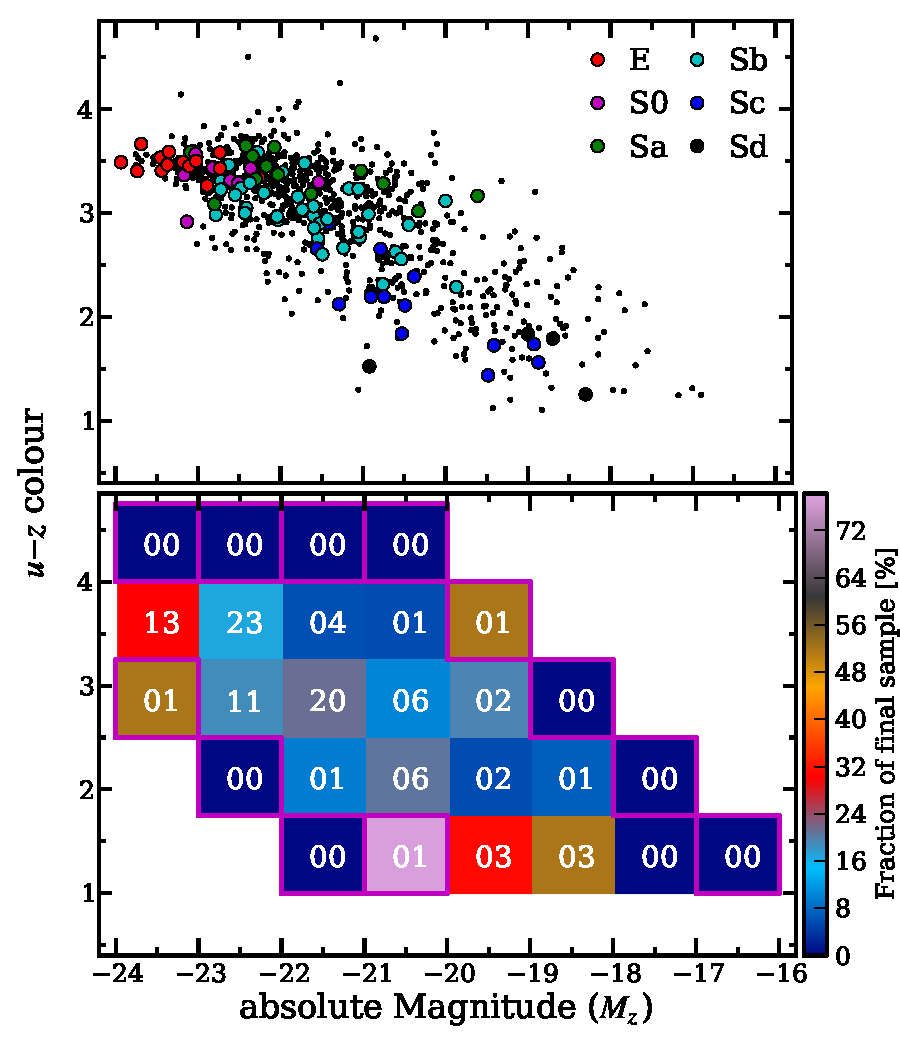
\includegraphics[height=0.5\textwidth]{figuras/figHusemann2013Fig2.pdf}
    \caption[Diagrama cor-magnitude para as galáxias do CALIFA.]
    {Distribui\c{c}\~ao das galáxias do CALIFA no diagrama cor magnitude $u-z$ vs. $M_z$. {\em
    Painel superior}: Em pontos pretos est\~ao as galáxias pertencente a amostra-m\~ae e em cores
    as galáxias presentes no CALIFA DR1. As diferentes cores representam os diferentes tipos
    morfológicos. {\em Painel inferior}: A fra\c{c}\~ao de galáxias observadas pelo DR1 em
    rela\c{c}\~ao a amostra-m\~ae. Retirado de \citet{Husemann.etal.2013a}.}
    \label{fig:cm-uzMz}
    \end{center}
\end{figure}

% bibliografia
\bibliographystyle{apj}
\bibliography{apj-jour,papers}

\vspace{2cm}

\signature[4in]{Roberto Cid Fernandes Jr. (Orientador)}

\vspace{2cm}

\signature[4in]{Eduardo Alberto Duarte Lacerda (Aluno)}

\vspace{4cm}

\begin{center}
Florianópolis, 16 de fevereiro de 2015.
\end{center}

\end{document}
